\documentclass{article}
\usepackage[paperwidth=20cm,paperheight=10cm,margin=0.4cm]{geometry}
\usepackage{tikz}
\usetikzlibrary{arrows.meta, positioning, calc, fit, backgrounds}
\usepackage[T1]{fontenc}
\usepackage{lmodern}
\usepackage{xcolor}
\pagestyle{empty}

% === Colors (customize per-figure) ===
\definecolor{boxA}{RGB}{210,228,248}
\definecolor{lineA}{RGB}{90,135,195}
\definecolor{boxB}{RGB}{255,230,200}
\definecolor{lineB}{RGB}{210,150,60}
\definecolor{iofill}{RGB}{245,245,245}
\definecolor{ioline}{RGB}{170,170,170}
\definecolor{arrcol}{RGB}{80,80,80}
\definecolor{sublabel}{RGB}{110,110,110}

% Sublabel helper: apply per-line, NOT inside braces around \\
\newcommand{\sub}[1]{\fontsize{7}{9}\selectfont\sffamily\color{sublabel}#1}

\begin{document}
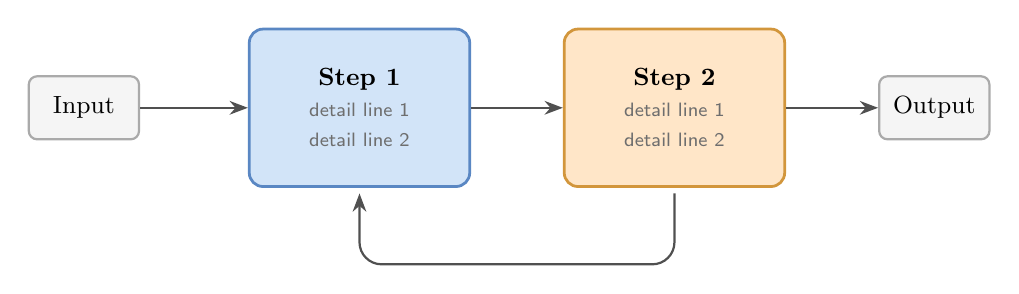
\begin{tikzpicture}[
  >=Stealth,
  boxA/.style={
    draw=lineA, fill=boxA, rounded corners=5pt, line width=1pt,
    minimum width=2.8cm, minimum height=2cm, align=center, font=\small
  },
  boxB/.style={
    draw=lineB, fill=boxB, rounded corners=5pt, line width=1pt,
    minimum width=2.8cm, minimum height=2cm, align=center, font=\small
  },
  iobox/.style={
    draw=ioline, fill=iofill, rounded corners=3pt, line width=0.8pt,
    minimum width=1.4cm, minimum height=0.8cm, align=center, font=\small
  },
  arr/.style={->, thick, color=arrcol},
]

% --- Example: simple flow ---
\node[iobox] (input) at (0,0) {Input};
\node[boxA]  (step1) at (3.5,0) {\textbf{Step 1}\\\sub{detail line 1}\\\sub{detail line 2}};
\node[boxB]  (step2) at (7.5,0) {\textbf{Step 2}\\\sub{detail line 1}\\\sub{detail line 2}};
\node[iobox] (output) at (10.8,0) {Output};

\draw[arr] (input) -- (step1);
\draw[arr] (step1) -- (step2);
\draw[arr] (step2) -- (output);

% --- Loop-back arrow ---
\draw[arr, rounded corners=8pt]
  ([yshift=-2pt]step2.south) -- ++(0,-0.9) -| ([yshift=-2pt]step1.south);

% --- Self-loop ---
% \draw[arr, rounded corners=8pt, line width=1.2pt]
%   ([xshift=5pt]step2.south) -- ++(0,-0.9) -| ([xshift=-5pt]step2.south);

% --- Dashed boundary ---
% \begin{scope}[on background layer]
%   \node[draw=black!30, dashed, rounded corners=8pt, inner sep=10pt,
%         line width=0.8pt, fit=(step2)] (boundary) {};
% \end{scope}
% \node[anchor=north, font=\fontsize{7}{8}\selectfont\sffamily, text=black!45]
%   at ([yshift=-4pt]boundary.south) {boundary label};

\end{tikzpicture}
\end{document}
